\documentclass[a4paper]{article}

\usepackage{interspeech2013,amssymb,amsmath,epsfig}
\setcounter{page}{1}
\sloppy		% better line breaks
\ninept
%SM below a registered trademark definition
\def\reg{{\rm\ooalign{\hfil
     \raise.07ex\hbox{\scriptsize R}\hfil\crcr\mathhexbox20D}}}

%% \newcommand{\reg}{\textsuperscript{\textcircled{\textsc r}}}
\title{Understanding the Perception of Courteous and Humorous Behavior using Prosodic and Lexical Features}

\makeatletter
\def\name#1{\gdef\@name{#1\\}}
\makeatother
\name{{\em Sidd Jagadish$^\ast$, Ranjay Krishna$^\ddagger$, Gabriele Carotti-Sha$^\mp$}}
\address{{\small \tt siddj@stanford.edu, rak248@stanford.edu, gcarotti@stanford.edu}\\
$^\ast$Department of Statistics, Stanford University \\
  $^\ddagger$Department of Computer Science, Stanford University\\
  $^\mp$ Symbolic Systems, Stanford University\\
}

%
\begin{document}
\maketitle
%

\begin{abstract}
Computationally understanding the perception of a speaker's characteristics is an important task speech processing, behavioral outcomes and dialogue systems. Our work focuses on the classification and understanding the perception of two such characteristics: courtesy and humor. We analyze ratings surveyed from the SpeedDate corpus to build models using prosodic and lexical features of the speakers. We find that lexical features like \textit{Hedge-words} and prosodic features like \textit{Intensity Min SD} are important for detecting courteous while \textit{Exclamations} and listener's \textit{Intensity} are important for funny. Using an Adaboost Classifier, we detect the funny with an accuracy of SHIT GOES HERE and courteous at SHIT GOES HERE.\\

\end{abstract}

\noindent{\bf Index Terms}: Prosody, Speed Date, AdaBoost, Gender differences in prosody, factor analysis, courteous, funny

%

\section{Introduction}

\section{Related Works}


\section{The SpeedDate Dataset}
We utilize the SpeedDate dataset introduced by \cite{jurafsky} to build our model. The dataset contains approximately 1100 heterosexual 4-minute speed dates. Each date is stored as a wav file recording of the speed date along with text files of the dates annotations. On average, each date contains 
812 words, with an average of 406 words per speaker. These worded are divided into an average of 93 turns per date where the speaker changes to the other.

\subsection{Feature Extraction}
We use OpenSMILE to extract Prosodic features from audio files of the speed date. Lexical features are extracted from the transcripts with the help of the LIWC dictionary.

\subsubsection{Prosodic Feature}
Prosodic features describe the speech of the speaker. In our model, we include features such as \textit{F0, intensity, RMS Amplitute, turn duration} and \textit{pitch}. For each of these different features, we calculate the \textit{min, max, sd, range, sd sd} and \textit{mean}.

\subsubsection{Lexical Feature}
Using LIWC, introduced by \cite{pennebaker}, we extract \textit{hedge words} like \textit{sort of} and \textit{I guess} that indicate uncertainty. We also gather \textit{meta} words that represent common words in the given speed date scenario and \textit{academic} words like \textit{PhD} and \textit{research}. Finally, we record occurrences of discourse markers.

\subsubsection{LIWC Feature}
We use the LIWC software to classify words into specific topic groups like \textit{love, hate, food, negate} and \textit{drink}. We count the word occurrences within each speed date for each of these word topics.

\subsubsection{Accomodation Feature}
\cite{natale}, \cite{ireland} and \cite{levitan} demonstrate through their work the convergence of vocal intensities between interlocutors. To capture this convergence, we extract features from a speaker that accommodate the previous speaker's speech. These features include the \textit{Rate of Speech} of the two speakers over time, the number of \textit{functional} and \textit{content} words also used in the other's previous turn and \textit{laughter} that immediately proceeds the other's laugh.

\subsection{Feature Normalization}
Before we use the features in our model, we normalize the relevant lexical feature with the the total word count in the conversation. We then normalize all the features such that they all have zero mean and unit variance.

\section{Exploratory Analysis}
Before attempting to classify speakers as funny or not, we examine the underlying dimensions along which the data varies.  To do, so we use exploratory factor analysis. To determine the number of factors, we use a scree test and various non-graphical measures, including parallel analysis and an optimal coordinates test, as described in (CITE).  We find an optimal number of factors $k = 5$ for both males and females, conducted separately.  Figure~\ref{scree} shows the two scree plots.

\begin{figure}[t]
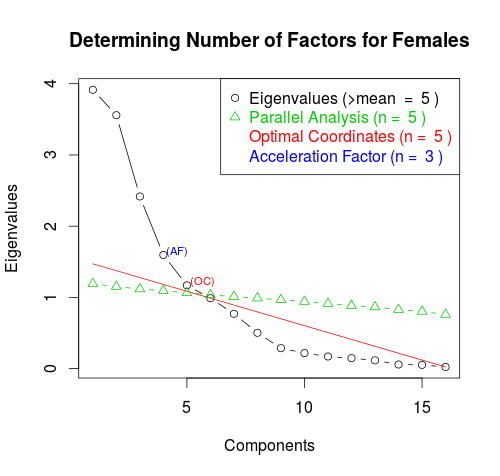
\includegraphics[width = 3.5cm]{graphics/ScreeFem.png}
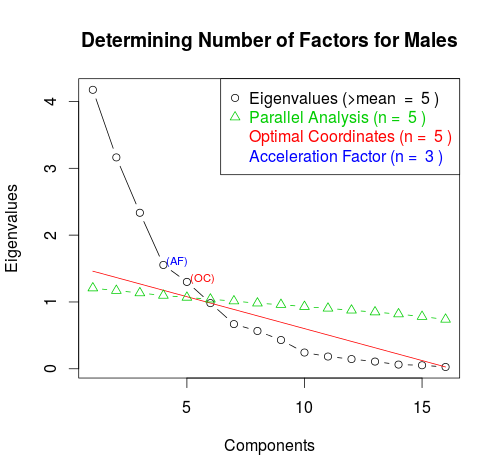
\includegraphics[width = 3.5cm]{graphics/ScreeMale.png}
\caption{{\it Determining Number of Factors}\label{scree}}  
\label{scree}
\end{figure}

Interestingly, although we find that the various factors for male and female speech are similar, they explain different amounts of variation in the data.  For males, the first factor reflects high intensity values and low intensity variation, explaining   

\section{Evaluation Approach}

\subsection{Methodology}
We divide the dataset into two separate groups based on gender. For each gender, we train a classifier for detecting the perception of funny and courteous characteristics.  

We create a training set for a given characteristic for a given gender by splitting the dataset into deciles. We use the top decile as positive and the bottom decile as negative examples. 

\subsection{Classifiers}
We start by using an SVM with a linear kernel. To improve our classifications, we next enforce an L1 norm on the SVM to compensate for the large number of lexical and prosodic features we extract. In case our decision boundaries are non-linear, we also train a RBF kernelized SVM. However, we lose interpretability of the features by using an RBF. So, we train a fourth Adaboost Classifier with decision stumps of unary depth to maintain interpretability while also allowing for a non-linear decision boundary.  

\section{Classification Results}

\section{Analysis}


\section{Future Work}


\section{Conclusions}


\section{Acknowledgements}
We thank Dan Jurafsky for giving us access to the Speed Dating Dataset and for his continued guidance during this project.

\newpage
%
\eightpt
\bibliographystyle{IEEEtran}
\begin{thebibliography}{10}

\bibitem{jurafsky}Ranganatha, R., Jurafsky, D., McFarland, D.A., ``Detecting friendly, flirtatious, awkward, and assertive speech in speed-dates``, in Computer Speech \& Language
Volume 27, Issue 1, Pages 89-115, 2013

\bibitem{pennebaker}Pennebaker, J. W., Booth, R., Francis, M., ``Linguistic inquiry and word count: LIWC2007`` � operator�s manual. Tech. rep., University of Texas, 2007

\bibitem{natale}Natale, M.,  ``Convergence of mean vocal intensity in dyadic communication as a function of social desirability``, in Journal of Personality and
Social Psychology 32 (5), 790-804, 1975

\bibitem{ireland}Ireland, M.E., Slatcher, R.B., Eastwick, P.W., Scissors, L.E., Finkel, E.J., Pennebaker, J.W., ``Language style matching predicts relationship
initiation and stability``, in Psychological Science 22 (1), 39, 2011

\bibitem{levitan}Levitan, R., Hirschberg, J., ``Measuring acoustic-prosodic entrainment with respect to multiple levels and dimensions``, in ACL 2011

\end{thebibliography}
\end{document}
